% questions.tex —— 1986 年·广东卷·理工农医类 · 题目内容片段（无答案）
% 由 tools/generate_projects.py 依来源总账自 1986/1986_数学真题_广东理_试题.md 生成，勿手改（改源 MD 后重跑）


\gkpart{广东省数学（理工农医类）}

\begin{gktip}
\textbf{来源说明}：本题面依据固定源 PDF《1986 年全国普通高等学校招生统一考试广东省数学（理工农医类）》PDF 第 1—6 页逐题转录，固定源页脚原卷页码为 30—32；PDF 第 7—11 页为答案和解答。固定源为扫描 PDF，题面以试题页为唯一来源，答案和解析由本库独立复算，不声称代表官方发布版本。

\textbf{版式与异文说明}：第 9 题的“幅角的主值”按固定源选项及答案表所反映的 $[0,2\pi)$ 约定记录为 $\frac{11\pi}{6}$；若采用现代常见的 $(-\pi,\pi]$ 约定，则写作 $-\frac\pi6$。第 12、15 题的末项选项标签在固定源中均出现重复字母，照录。第 8、9 题等若干乘法位置显示为方框缺字形，照录为 $\square$。第 25 题图形选项区域在固定源中完全空白，保留题干和答案表信息，不凭空补画。

\textbf{图形说明}：第二卷第二题（三棱锥）图形依据固定源关系重绘为 TikZ 矢量图。
\end{gktip}

\begin{question}
\gkti{1}（本题满分 50 分）本题共有 25 个小题。每一个小题都给出代号为 $A\text{、}B\text{、}C\text{、}D\text{、}E$ 的五个结论，其中只有一个结论是正确的。请把正确结论的代号选出，并在答题卷中的相应位置上涂黑（每个小题选对得 2 分，不选、选错或者选出的代号超过一个，一律得 0 分）。

（1） 通过点 $(0,2)$ 且倾斜角为 $15^\circ$ 的直线的方程是\mbox{（　　）}

（A）$y=(\sqrt3-2)x+2$　　（B）$y=(\sqrt2-1)x+2$

（C）$y=(2-\sqrt3)x+2$　　（D）$y=(\dfrac{\sqrt3}{2}-1)x+2$

（E）$y=(\sqrt3-1)x+2$

（2） 设 $\alpha,\beta\in(0,\frac\pi2)$ 且 $\operatorname{tg}\alpha=\frac43,\operatorname{tg}\beta=\frac17$，则 $\alpha-\beta=$\mbox{（　　）}

（A）$\dfrac\pi3$　　（B）$\dfrac\pi4$　　（C）$\dfrac\pi6$　　（D）$\dfrac\pi8$　　（E）$-\dfrac\pi3$

（3） 侧面为等边三角形的正三棱锥，其侧面与底面所成的二面角的余弦的值是\mbox{（　　）}

（A）$\dfrac{\sqrt3}{2}$　　（B）$\dfrac{\sqrt2}{2}$　　（C）$\dfrac12$　　（D）$\dfrac13$　　（E）$\dfrac{\sqrt2}{3}$

\Needspace{5\baselineskip}
（4） 参数方程

\nopagebreak[4]
\[
\begin{cases}
x=1-2\sin\varphi,\\
y=\cos\varphi
\end{cases}
\qquad(\varphi\text{ \text{为参数}})
\]

所表示的曲线是\mbox{（　　）}

（A）圆　　（B）焦点在 $x$ 轴上的双曲线　　（C）焦点在 $y$ 轴上的双曲线

（D）焦点在 $x$ 轴上的椭圆　　（E）焦点在 $y$ 轴上的椭圆

（5） 复数 $\sin95^\circ+i\cos95^\circ$ 的一个辐角是\mbox{（　　）}

（A）$-85^\circ$　　（B）$-5^\circ$　　（C）$5^\circ$　　（D）$85^\circ$　　（E）$95^\circ$

（6） 若复数 $(\sqrt3+i)^n$ 是一个纯虚数，则 $n$ 的一个可能的值是\mbox{（　　）}

（A）5　　（B）6　　（C）7　　（D）8　　（E）9

（7） 在复平面上，设动点 $Z$ 对应的复数为 $z$，$Z$ 到复数 $-i$ 和 $1+i$ 所对应的点的距离之和等于 5，则动点 $Z$ 的轨迹方程是\mbox{（　　）}

（A）$|z+i|+|z-1-i|=5$　　（B）$|z-i|+|z+1+i|=5$

（C）$(z+i)+(z-1-i)=5$　　（D）$(z-i)+(z+1+i)=5$

（E）$(z+i)^2+(z-1-i)^2=25$

（8） 要从 8 名男医生和 7 名女医生中选 5 人组成一个医疗小组，如果医疗小组中至少有 2 名男医生和至少有 2 名女医生，则不同选法的种数是\mbox{（　　）}

（A）$(C_8^3+C_7^2)\square(C_7^3+C_8^2)$

（B）$(C_8^3+C_7^2)+(C_7^3+C_8^2)$

（C）$C_8^2\square C_7^3$　　（D）$C_8^2\square C_7^2\square C_{11}^1$

（E）$C_8^2\square C_7^3+C_8^3\square C_7^2$

（9） 要排一张有 5 个独唱节目和 3 个合唱节目的演出节目表，如果合唱节目不排头，并且任何两个合唱节目不相邻，则不同排法的种数是\mbox{（　　）}

（A）$P_8^8$　　（B）$P_5^5\square P_3^3$　　（C）$P_5^5\square P_5^3$

（D）$P_5^5\square P_8^3$　　（E）$P_8^5\square P_8^3$

（10） 设 $a,b$ 为实数且 $a+b=3$，则 $2^a+2^b$ 的最小值是\mbox{（　　）}

（A）6　　（B）$4\sqrt2$　　（C）$2\sqrt2$　　（D）$2\sqrt6$　　（E）8

\Needspace{5\baselineskip}
（11） 若 $\operatorname{ctg}\theta=3$，则

\nopagebreak[4]
\[
\cos^2\theta+\frac12\sin2\theta
\]

的值是\mbox{（　　）}

（A）$-\dfrac65$　　（B）$-\dfrac45$　　（C）$\dfrac45$　　（D）1　　（E）$\dfrac65$

\Needspace{5\baselineskip}
（12） 若 $\theta\in(\frac{5\pi}4,\frac{3\pi}2)$，则

\nopagebreak[4]
\[
\sqrt{1-\sin2\theta}
\]

等于\mbox{（　　）}

（A）$\cos\theta-\sin\theta$　　（B）$\sin\theta+\cos\theta$

（C）$\sin\theta-\cos\theta$　　（D）$-\cos\theta-\sin\theta$

（D）$|\cos\theta|-|\sin\theta|$

\Needspace{5\baselineskip}
（13） 函数

\nopagebreak[4]
\[
y=\cos x-\sin^2x-\cos2x+\frac74
\]

的最大值是\mbox{（　　）}

（A）$\dfrac74$　　（B）2　　（C）$\dfrac94$　　（D）$\dfrac{17}4$　　（E）$\dfrac{19}4$

\Needspace{5\baselineskip}
（14） 计算下式：

\nopagebreak[4]
\[
\operatorname{arctg}(1-\sqrt2)
\]

等于\mbox{（　　）}

（A）$-\dfrac{5\pi}8$　　（B）$-\dfrac{3\pi}8$　　（C）$-\dfrac\pi8$

（D）$\dfrac\pi8$　　（E）$\dfrac{3\pi}8$

\Needspace{5\baselineskip}
（15） 椭圆

\nopagebreak[4]
\[
\frac{(x+1)^2}{4}+y^2=1
\]

\Needspace{5\baselineskip}
与抛物线

\nopagebreak[4]
\[
y=1-(x+1)^2
\]

的交点的个数是\mbox{（　　）}

（A）0　　（B）1　　（C）2　　（D）3　　（D）4

\Needspace{5\baselineskip}
（16） 若动圆与圆

\nopagebreak[4]
\[
(x+2)^2+y^2=4
\]

相外切且与直线 $x=2$ 相切，则动圆的圆心的轨迹方程是\mbox{（　　）}

（A）$y^2-12x+12=0$　　（B）$y^2+12x-12=0$　　（C）$y^2+8x=0$

（D）$y^2-8x=0$　　（E）$y^2-6x+6=0$

\Needspace{5\baselineskip}
（17） 通过点 $A(3,4)$ 及双曲线

\nopagebreak[4]
\[
\frac{x^2}{6}-\frac{y^2}{3}=1
\]

的两个焦点的圆的方程是\mbox{（　　）}

（A）$x^2+(y-\frac83)^2=\frac{145}{9}$　　（B）$(x-\frac83)^2+y^2=\frac{145}{9}$

（C）$(x-2)^2+y^2=13$　　（D）$x^2+(y-2)^2=13$　　（E）$x^2+(y-\frac{11}4)^2=\frac{169}{16}$

\Needspace{5\baselineskip}
（18） 函数

\nopagebreak[4]
\[
y=\sqrt{x^2+2x-3}
\]

的单调下降区间是\mbox{（　　）}

（A）$(-\infty,-3]$　　（B）$[-3,+\infty)$　　（C）$(-\infty,-1]$

（D）$[-1,+\infty)$　　（E）$[-3,-1]$

\Needspace{5\baselineskip}
（19） 函数

\nopagebreak[4]
\[
y=\log_{\cos1}(\cos x)
\]

的值域是\mbox{（　　）}

（A）$[-1,1]$　　（B）$(-\infty,+\infty)$　　（C）$(-\infty,0]$

（D）$[0,+\infty)$　　（E）$[\cos1,(\cos1)^{-1}]$

（20） 在空间中，下列命题中成立的是\mbox{（　　）}

（A）过平面 $\alpha$ 外的两点，必有且只有一个平面与平面 $\alpha$ 垂直。

（B）若直线 $l$ 上有两点到平面 $\alpha$ 的距离相等，则直线 $l$ 必平行于平面 $\alpha$。

（C）若直线 $l$ 与平面 $\alpha$ 内的无数多条直线垂直，则直线 $l$ 必垂直于平面 $\alpha$。

（D）互相平行的两条直线在一个平面内的射影必然是互相平行的两条直线。

（E）若点 $P$ 到三角形的三条边的距离相等，则点 $P$ 在该三角形所在平面内的射影必然是三角形的内心。

（21） 四棱锥成为正四棱锥的一个充分但不必要的条件是\mbox{（　　）}

（A）各侧面是等边三角形　　（B）底面是正方形

（C）各侧面三角形的顶角是 $45^\circ$　　（D）各侧面是等腰三角形且底面为正方形

（E）顶点到底面的射影在底面四边形对角线的交点上

\Needspace{5\baselineskip}
（22） 设有函数

\nopagebreak[4]
\[
\text{① }y=\cos\frac{x+3\pi}{2},\qquad
\text{② }y=\sin\frac{x+5\pi}{2},
\]

则\mbox{（　　）}

（A）①与②都是奇函数　　（B）①与②都是偶函数

（C）①是奇函数而②是偶函数　　（D）①是偶函数而②是奇函数

（E）①与②中至少有一个既不是奇函数也不是偶函数

\Needspace{5\baselineskip}
（23） 设函数

\nopagebreak[4]
\[
y=\operatorname{tg}(\operatorname{arctg}\,2x),\qquad
y=\operatorname{arctg}(\operatorname{tg}\,2x),
\]

\Needspace{5\baselineskip}
与

\nopagebreak[4]
\[
y=\sin(\arcsin 2x)
\]

的图象分别记为 $l_1,l_2,l_3$，则\mbox{（　　）}

（A）$l_1,l_2,l_3$ 都相同　　（B）只有 $l_1$ 与 $l_2$ 相同

（C）只有 $l_1$ 与 $l_3$ 相同　　（D）只有 $l_2$ 与 $l_3$ 相同

（E）$l_1,l_2,l_3$ 都不相同

（24） 若点 $A$ 的坐标为 $(3,2)$，$F$ 为抛物线 $y^2=2x$ 的焦点，点 $P$ 在该抛物线上移动，为使 $|PA|+|PF|$ 取最小值，点 $P$ 的坐标应为\mbox{（　　）}

（A）$(0,0)$　　（B）$(1,1)$　　（C）$(2,2)$　　（D）$(\frac12,1)$　　（E）$(1,\sqrt2)$

\Needspace{5\baselineskip}
（25） 若函数 $y=f(x)$ 是函数

\nopagebreak[4]
\[
y=1-\sqrt{1-x^2},\qquad -1\le x\le0
\]

的反函数，则 $y=f(x)$ 的图象大致形状是\mbox{（　　）}

\begin{gktip}
固定源第 4 页题干之后的 A—E 图形选项区域完全空白。本文只保留题干和固定源答案表记录，不凭空补画图形。
\end{gktip}

\end{question}
\begin{question}
\gkti{2}（本题满分 30 分）本题共有 10 个小题，每一个小题满分 3 分，只要求直接写出结果。

\Needspace{5\baselineskip}
（1） 函数

\nopagebreak[4]
\[
y=2\log_3x\qquad(x>0)
\]

的反函数是 $\underline{\hspace{2em}}$。

\Needspace{5\baselineskip}
（2） 将极坐标方程

\nopagebreak[4]
\[
\rho=\operatorname{tg}\theta\ \square\ \sec\theta
\]

化为直角坐标方程，得 $\underline{\hspace{2em}}$。

\begin{gktip}
固定源中的乘法位置显示为方框缺字形 $\square$，按题意解释为乘法，但题面记录不替换该字形。
\end{gktip}

\Needspace{5\baselineskip}
（3） 若球内切于圆柱，则它们的表面积之比

\nopagebreak[4]
\[
S_{\text{\text{圆柱全}}}:S_{\text{\text{球}}}
\]

的值是 $\underline{\hspace{2em}}$。

\Needspace{5\baselineskip}
（4） 中心在原点的双曲线，若其实半轴长为 2，一条准线的方程为

\nopagebreak[4]
\[
x=-\frac12,
\]

则该双曲线的离心率的值是 $\underline{\hspace{2em}}$。

\Needspace{5\baselineskip}
（5） 设函数 $y=\lg(x^2-x-2)$ 的定义域为 $A$，函数

\nopagebreak[4]
\[
y=\sqrt{\frac{x+2}{1-x}}
\]

的定义域为 $B$，则 $A\cap B=$ $\underline{\hspace{2em}}$。

\Needspace{5\baselineskip}
（6） 已知等差数列 $\{a_n\}$ 的公差是正数，且

\nopagebreak[4]
\[
a_3a_7=-12,\qquad a_4+a_6=-4,
\]

则前 20 项的和 $S_{20}=$ $\underline{\hspace{2em}}$。

\Needspace{5\baselineskip}
（7） 计算下式：

\nopagebreak[4]
\[
(2x-1)^5
\]

的展开式中各项系数的绝对值的和为 $\underline{\hspace{2em}}$。

\Needspace{5\baselineskip}
（8） 求极限：

\nopagebreak[4]
\[
\lim_{n\to\infty}\sqrt n\left(\sqrt{n+1}-\sqrt n\right)
=\underline{\hspace{2em}}\text{。}
\]

\Needspace{5\baselineskip}
（9） 方程

\nopagebreak[4]
\[
\sin\left(\frac\pi3-x\right)\ \square\
\cos\left(x+\frac\pi3\right)-\frac{\sqrt3}{2}=0
\]

的解集是 $\underline{\hspace{2em}}$。

\begin{gktip}
固定源中两个三角函数之间的乘法位置显示为方框缺字形 $\square$，按题意解释为乘法，但题面记录不替换该字形。
\end{gktip}

\Needspace{5\baselineskip}
（10） 当 $a$ 在 $(-\infty,0)$ 内变化时，要使过三点

\nopagebreak[4]
\[
O(0,0),\qquad A(-4,0),\qquad B(-2,a)
\]

的圆的圆心在 $\triangle AOB$ 内（包括边界），则 $a$ 允许取的最大值是 $\underline{\hspace{2em}}$。

\end{question}
\begin{question}
\gkti{3}（本题满分 8 分）设有对数方程

\nopagebreak[4]
\[
\lg(ax)=2\lg(x-1).
\]

（1） 当 $a=2$ 时，解该对数方程；

（2） 证明：当 $a>0$ 时，该对数方程有且只有一个解，并求出它的解。

\Needspace{0.4\textheight}
\end{question}
\begin{question}
\gkti{4}（本题满分 12 分）在三棱锥 $S-ABC$ 中，平面 $SAC\perp ABC$，$AB=AC=a$，$\angle BAC=90^\circ$，$SA=SC=b$。求：

（1） 棱 $SB$ 与平面 $ABC$ 所成角的正切；

（2） 三棱锥被过 $S$ 且与 $BC$ 垂直的平面所截得的截面面积。
\nopagebreak[4]
\begin{center}% 1986 年广东卷理工农医类第 4 题：三棱锥
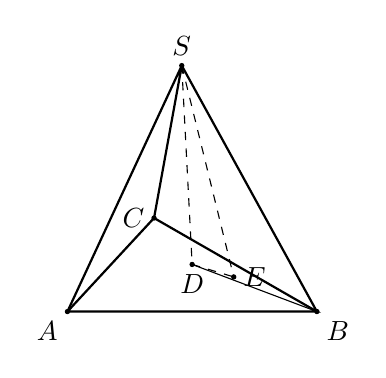
\begin{tikzpicture}[scale=0.88,>=stealth]
  \coordinate (A) at (0,0);
  \coordinate (B) at (3.6,0);
  \coordinate (C) at (1.25,1.35);
  \coordinate (S) at (1.65,3.55);
  \coordinate (D) at (1.8,0.68);
  \coordinate (E) at (2.4,0.5);

  \draw[thick] (A)--(B)--(C)--cycle;
  \draw[thick] (S)--(A) (S)--(B) (S)--(C);
  \draw[dashed] (A)--(C);
  \draw[dashed] (S)--(D) (S)--(E) (D)--(E);
  \draw (D)--(B);
  \fill (A) circle (1.1pt) node[below left] {$A$};
  \fill (B) circle (1.1pt) node[below right] {$B$};
  \fill (C) circle (1.1pt) node[left] {$C$};
  \fill (S) circle (1.1pt) node[above] {$S$};
  \fill (D) circle (1.1pt) node[below] {$D$};
  \fill (E) circle (1.1pt) node[right] {$E$};
\end{tikzpicture}
\end{center}
\nopagebreak[4]
\end{question}
\begin{question}
\gkti{5}（本题满分 12 分）设

\nopagebreak[4]
\[
a_n=\cos n\alpha,\qquad 0<\alpha<\pi.
\]

（1） 试用 $a_{n-1},a_{n-2}$ 表示 $a_n$；

\Needspace{5\baselineskip}
（2） 用数学归纳法证明

\nopagebreak[4]
\[
a_1+a_2+\cdots+a_n
=\frac{\sin\frac{n\alpha}{2}\cos\frac{(n+1)\alpha}{2}}
{\sin\frac\alpha2};
\]

\Needspace{5\baselineskip}
（3） 求

\nopagebreak[4]
\[
a_1-a_2+a_3-a_4+\cdots+(-1)^{k+1}a_k+\cdots-a_{2n}+a_{2n+1}.
\]

\end{question}
\begin{question}
\gkti{6}（本题满分 12 分）已知椭圆 $C$ 的直角坐标方程为

\nopagebreak[4]
\[
\frac{x^2}{4}+\frac{y^2}{3}=1,
\]

\Needspace{5\baselineskip}
试确定 $m$ 的取值范围，使得对于直线

\nopagebreak[4]
\[
y=4x+m,
\]

椭圆 $C$ 上有不同的两点关于该直线对称。

\end{question}